\section{Experimental results} \label{sec:results}

% Past Tense

\begin{comment}
  - Introduction: What is expected
  - Global Numbers
  - Different Band (Noise)
  - Precision/Recall Graphs
  - Histograms Recall, Precision and F-Score
  
  - Noticeable changes in results
  - Different Width (variable fwmh)
  - Marginal changes in results
  - Border cases not resolved
\end{comment}

%  Introduction: What is expected
In this section, we present and analyze the experimental results obtained.
The idea behind the tests is to simulate data cubes using a known isotope list and then, to retrieve of as much elements of the known list as possible.
For each band, the list of all theoretical isotopes in that range are searched in Splatalogue, and a subset of them is selected randomly to simulate data cubes.

\subsection{Measure of accuracy}
To evaluate identification performance, a measure of test accuracy must be design such that we can evaluate percentage of matches between selected words and present lines in simulations.
% Histograms Recall, Precision and F-Score
We use as measures precision, recall and f-score in view of its intuitive ability to explain performance differentiating accuracy from true/false positives/negatives \citep{precision_recall}.
F-score values in table \ref{tab:results} show an overview of obtained results.

Moreover, confusion matrices in figure \ref{fig:confusion_matrix} allow to visually analyze the classifier performance.
The matrices, that corresponds to first 20 experiments at ALMA band 9, show that predictions become less certain at darker zones.
Confusion matrices tends to be higher than wider because of the greater number of false positive predictions over actual isotope lines.
Indicators of performance precision, recall and f-score are calculated from their respective confusion matrices.
The precision/recall curves are shown at figures \ref{fig:results1} and \ref{fig:results2} for ALMA bands 9 and 7 respectively.

\subsection{Prediction results}
Overall results give a f-score above 90\% when the results are filtered for cases in which the lines present in the simulation are higher than 1 MHz.
One might expect higher results in such that cases, but the fact that present lines are not closer does not necessarily simplifies the task.
Theoretical lines keep being very close for some cases and an error margin is expected.

When all results are included, an overall f-score of 82\% is reached, showing that the idea behind this approach is suitable to solve the problem.
In next sections, we will address differences between each group of results.

% Table with Results
\begin{center}
	\begin{table}
		\begin{tabular}{ | l | l | l | }
			\hline
			{\bf ALMA Band/Width } & {\bf Fixed } & {\bf Variable} \\ \hline
			Band 7 & 85.80 \% & 84.79 \% \\ \hline
			Band 9 & 82.05 \% & 78.17 \% \\ 
			\hline
		\end{tabular}
		\caption{ The f-score for different noise level (bands) and width of the lines.}
		\label{tab:results}
	\end{table}
\end{center}

% Noticeable changes in results
\subsection{Signal to noise effect in predictions}
There exists noticeable differences between results for different noise levels.
For band 9, an overall of 80\% shows that both the higher noise and density affect prediction accurately.
On the other hand, band 7 reaches an overall of 85\%, although there are not appreciable differences between the measures distribution as can be seen in both figures \ref{fig:hist1} and \ref{fig:hist2}.

Figures \ref{fig:results1} and \ref{fig:results2} show an intuition of exchange ratio between true positive and false negatives.
Precision/recall curve at band 7 has a better trade-off as its slope is smaller,  and this is reflected in better prediction of true positives without increasing false positives.

\subsection{Variable width effect in predictions}
% Different Width (variable fwmh)
To test more realistic cases, where line width variates randomly, there is a small difference of almost 1\% for band 7.
Not so at band 9, where a difference of 4\% shows that higher density of lines is affected by the randomness of lines's width.
Also, figures \ref{fig:hist1} and \ref{fig:hist2} shows the differences between accuracy measures for both cases, being the fixed width focused in a smaller range than variable width results.

% Example of Modified Confusion Matrix
\begin{figure}
	\begin{center}
		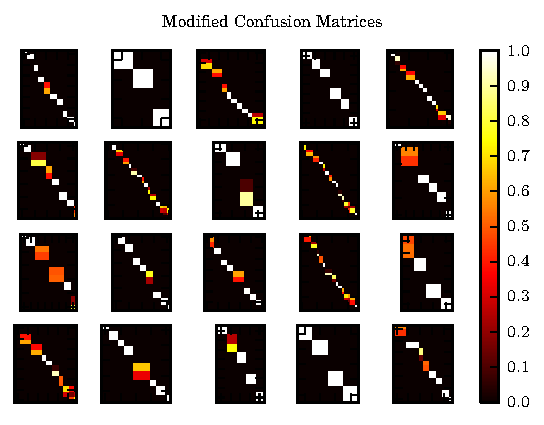
\includegraphics[width=0.45 \textwidth]{images/confusion_matrix}
		\caption{ Modified confusion matrices for 20 experiments for data cubes with fixed line width at band 9. Predictions tend to be on the diagonal because of the algorithm preference for closer theoretical line's frequencies.}
		\label{fig:confusion_matrix}
	\end{center}
\end{figure}

% Precision/Recall Curve
\begin{figure}[H]
	\begin{center}
		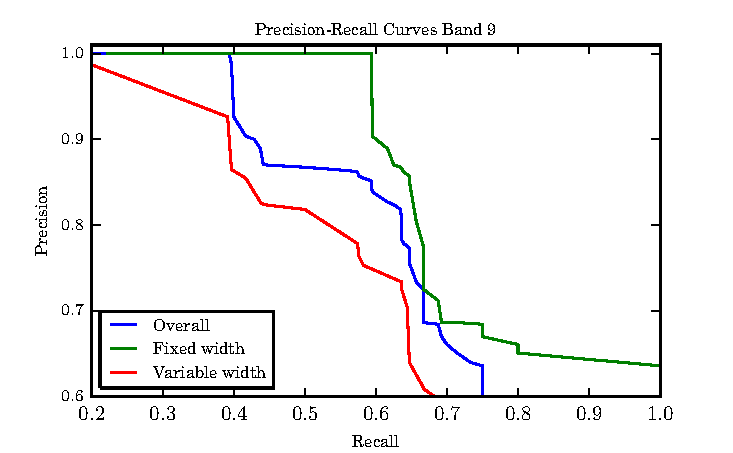
\includegraphics[width=0.45\textwidth]{images/results1}
		\caption{ The measures of accuracy, precision and recall obtained for fixed line width cubes, variable line width and overall results for ALMA band 9.}
		\label{fig:results1}
	\end{center}
\end{figure}

\begin{figure}[H]
	\begin{center}
		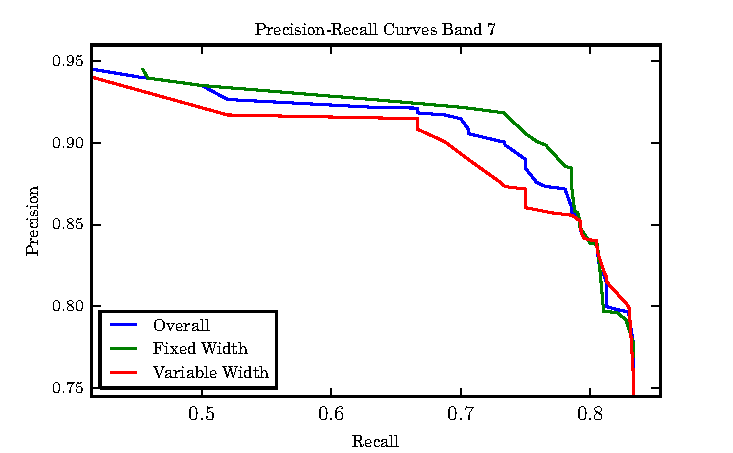
\includegraphics[width=0.45\textwidth]{images/results2}
		\caption{ The measures of accuracy, precision and recall obtained for fixed line width cubes, variable line width and overall results for ALMA band 7. }
		\label{fig:results2}
	\end{center}
\end{figure}

% Histograms of results Fixed Width
\begin{figure}[H]
	\begin{center}
		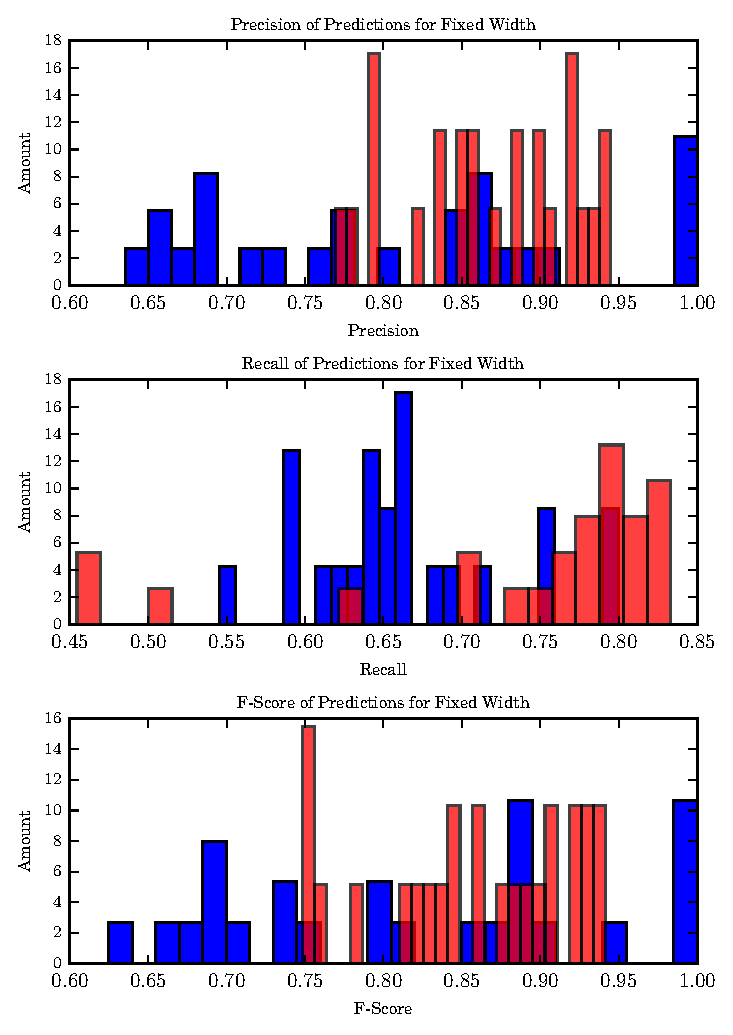
\includegraphics[width=0.45\textwidth]{images/hist1}
		\caption{ Histograms of results obtained for the test performed for precision, recall and f-score for fixed line width (red) vs variable line width (blue) in Band 9.}
		\label{fig:hist1}
	\end{center}
\end{figure}

\subsection{Complex cases}
%  %  Blending case
We focus our analysis on complex cases and show examples of how the algorithm handle them.

For blending cases, the algorithm gives a probability distribution of potential overlapped lines. In general, when blending exists, one of the predicted lines losses certainty, as showed in figure \ref{fig:blending}.

\begin{figure}[H]
	\begin{center}
		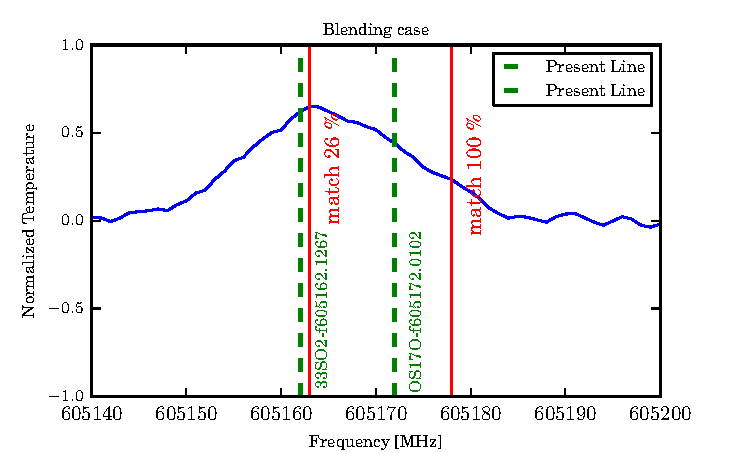
\includegraphics[width=0.45\textwidth]{images/blending}
		\caption{ Blending case }
		\label{fig:blending}
	\end{center}
\end{figure}

% Histograms of results Variable Width
\begin{figure}[H]
	\begin{center}
		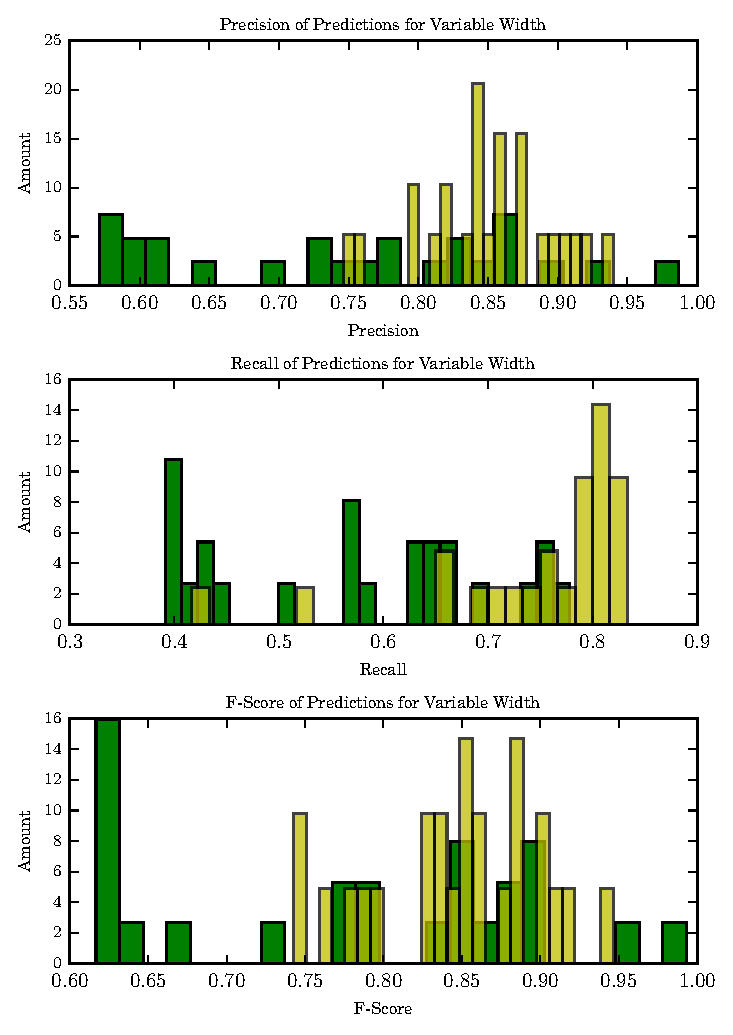
\includegraphics[width=0.45\textwidth]{images/hist2}
		\caption{ Histograms of results obtained for the test performed for precision, recall and f-score for fixed line width (yellow) vs variable line width (green) in Band 7.}
		\label{fig:hist2}
	\end{center}
\end{figure}


% Double peaks for single Line
False double peaks product of artifacts are handled by the algorithm and it determines the correct lines among false peaks, as showed in figure \ref{fig:doublepeak}.

\begin{figure}[H]
	\begin{center}
		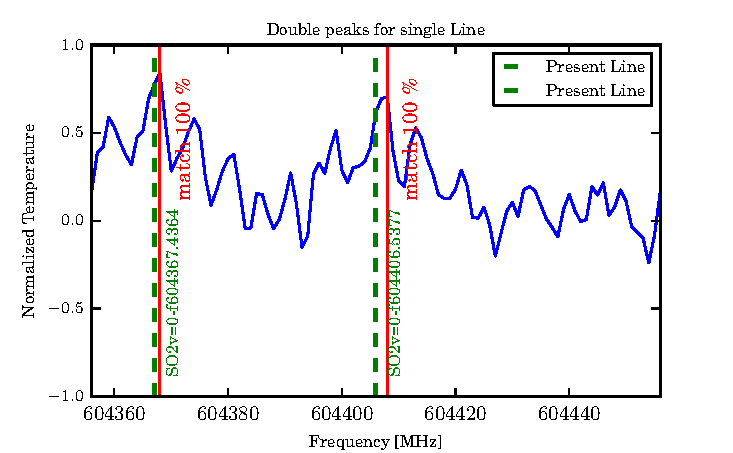
\includegraphics[width=0.45\textwidth]{images/doublepeak}
		\caption{ Double peaks for single Line }
		\label{fig:doublepeak}
	\end{center}
\end{figure}